\section{Von Neumannovy principy, blokové schéma Von Neumannova počítače. Rozdíl mezi Von Neumannovou, harvardskou a modifikovanou harvardskou architekturou. Procesory CISC a RISC. Rozdíl mezi obvodovým a mikroprogramovým řadičem. Řetězové zpracování instrukcí (pipelining), skokový a datový konflikt. Jak se liší a pro jaké typy úloh je určen mikroprocesor pro všeobecné použití, mikrokontrolér, signálový procesor a signálový kontrolér (DSC), SoC (System on a Chip), ASIC.}
\subsection{Von Neumnnova architektura}
\subsubsection*{Hlavní myšlenka}
Instrukce programu jsou reprezentovány binárními signály a jsou uloženy v paměti počítače spolu s daty. \\
\subsubsection*{Principy}
Principy:
\begin{itemize}
    \item Předpis pro řešení úlohy je převeden na posloupnost instrukcí
    \item Intrukce a data se nacházejí ve stejné paměti
    \item Instrukce ani data nejsou explicitně označeny
    \item Paměť je rozdělena na stejně velká paměťová místa nazývaná adresy
    \item V instrukcích není uvedena hodnota operandu, ale jeho adresa
    \item instrukce se provádějí sekvenčně
    \item Toto sekvenční provádění lze narušit instrukcemi typu skok
\end{itemize}

\begin{figure}[h!]
    \centering
    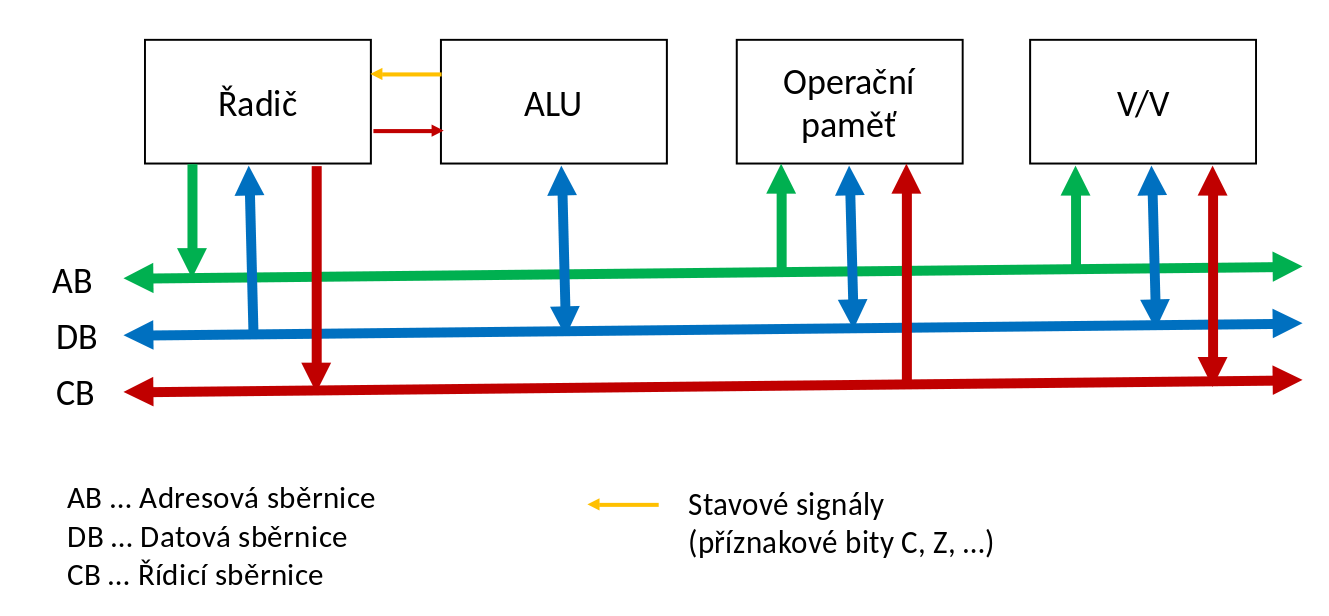
\includegraphics[width = \textwidth]{img/VonNeumann.png}
\end{figure}

\subsubsection*{Řadič}
Řídí činnost ostatních částí počítače. \\
Implementuje instrukční sadu. \\
Vstupy:\\
\begin{itemize}
    \item Signály z dekodéru instrukcí - dekóduje se část instrukce označována jako operační znak
    \item Signály generované ALU - Příznaky, přetečení, nulový výsledek, záporný výsledek
    \item Signál žádosti o obsluhu přerušení
\end{itemize}
Výstupy:\\
\begin{itemize}
    \item Čtení nebo zápis do paměti
    \item Čtení nebo zápis do periferie
    \item Signály ALU, určující kterou operaci má provést
\end{itemize}

\subsubsection*{ALU}
Aritmeticko-logická jednotka.\\
Provádí aritmetické operace(+,-,/,*), logické operace(AND,OR,NOT) a operace porovnání(>,<,=)\\
Řadič a ALU tvoří CPU. Integrací řadiče, ALU a registrů na jeden čip vzniká mikroprocesor.

\subsubsection*{Operační paměť}
Místo uložení dat a instrukcí.\\
Společná paměť pro instrukce a data. Jsou uloženy v jednom paměťovém prostoru.\\
U mikrokontrolerů jsou v instrukce v paměti FLASH a proměnné v paměti RAM, ale obě jsou připojeny ke stejným sběrnicím(AB,CB,DB)

\subsubsection*{V/V}
Slouží pro komunikaci s okolím.\\
Člověkem - klávesnice, myš, obrazovka. \\
Strojem, přístrojem či technologickým procesem - I/O, A/D, D/A převodníky a k nim akční členy - snímače. \\
S ostatními počítači a zařízeními pomocí sítě - Ethernet, WiFi moduly. \\
Umožňují ukládání dat na disky(SSD, HDD). \\

\subsubsection*{Registry}
Typy registrů:
\begin{itemize}
    \item Pracovní registr
          \begin{itemize}
              \item Ukládají operandy z ALU a výsledky z ALU
              \item Rychlejší než operační paměť
              \item Původně jeden registr nazývaný akumulátor
          \end{itemize}
    \item Stavový registr
          \begin{itemize}
              \item Skupina klopných obvodů ovládaných ALU
              \item Uchovávají stav ALU mezi instrukcemi
              \item Příznaky přetečení/výpůjčky, nulového či záporného výsledku
              \item Předcházející instrukce příznaky nastaví, následující využije
          \end{itemize}
    \item Programový čítač
          \begin{itemize}
              \item Zajišťuje sekvenční provádění instrukcí a provádění skoků
              \item V průběhu zpracování instrukce se nastaví tak aby obsahoval adresu následující instrukce
          \end{itemize}
\end{itemize}
Řídící a stavový registr bývají spojeny do jednoho řídícího stavového registru.\\

\subsubsection{Cyklus počítače}
Celý cyklus práce počítače se dělí na tyto opakující se části.
\begin{enumerate}
    \item Intruction fetch - načtení instrukce z paměti
    \item Intruction decode - dekódování instrukce
    \item Operand fetch - načtení operandu z registrů
    \item Intruction expectation
    \item Write-back (Result store) - uložení výsledku
    \item Test, není-li požadavek na přerušení
\end{enumerate}
Nemusí se nutně vykonávat všechny tyto fáze.\\
Povinné fáze jsou pouze 1,2,4.

\subsection{Rozdíly mezi VonNeumannovou, harvardskou a modifikovanou harvardskou architekturou}
\subsubsection*{Von Neumannova architektura}
Společná paměť pro instrukce a data. \\
Existuje jedna datová a jedna adresová sběrnice. \\
Pomalejší oproti HA a MHA kvůli nutnosti číst instrukce nebo operand. \\
Výhoda spouštění programů z disků, jednoduchá změna počítače. \\
Dobře využitelná paměť. \\
Poloviční počet sběrnic oproti HA. Jednodušší konstrukce. \\
\begin{figure}[h!]
    \centering
    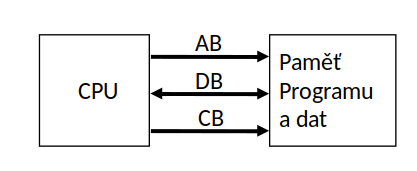
\includegraphics[]{img/VNporovnani.png}
\end{figure}

\subsubsection{Harvardská architektura}
Oddělena paměť dat a programu. To umožňuje číst obě zaráz a urychluje práci.\\
Může být různě adresována datová paměť a programová paměť.\\
Bezpečnější, nelze si poškodit program přepsáním jeho paměti.\\
Dvojnásobek sběrnic oproti VN, technilogicky velký problém. \\
Nevyužitou část paměti nejde použít pro program a naopak. Z toho plyne, že je nižší efektivita využití paměti. \\
Využívá se u signálových procesorů, jinak moc ne.\\
\begin{figure}[h!]
    \centering
    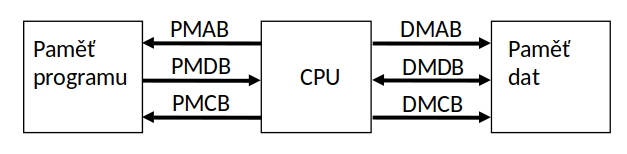
\includegraphics[width = \textwidth]{img/HAporovnani.png}
\end{figure}

\subsubsection*{Modifikovaná harvardská architektura}
Stejně jako HA 2 paměti. S rozdílem toho, že jedna je čistě pro data a druhá pro data a program.\\
Umožňuje číst 2 operandy zároveň díky rozmístění paměti. Toto umožňuje operaci Multiply and accumulate. \\
Využívá se u signálových procesorů a kontrolerů. \\

\begin{figure}[h!]
    \centering
    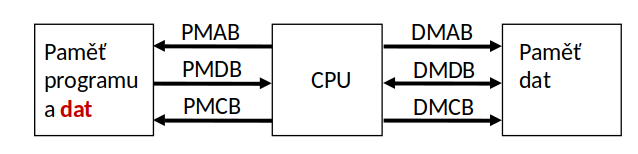
\includegraphics[width = \textwidth]{img/MHAporovnani.png}
\end{figure}

\subsection{Obvodový a mikroprogramový řadič}
\subsubsection*{Obvodový řadič}
Synchronní konečný stavový automat.\\
Logické členy a klopné obvody. \\
Umožňuje malou sadu jednoduchých instrukcí. \\
Výhodou je jednoduchost a malý počet součástek. \\
Nevýhodou je nutnost složité operace rozdělovat na více instrukcí. \\

\subsubsection*{Mikroprogramový řadič}
KSA, jehož paměť je tvořena pamětí mikroprogramu. \\
Implementuje složité instrukce za cenu složitosti řadiče. \\
Složité instrukce není možné přímo provést, proto jsou rozděleny na mikroinstrukce. \\
Posloupnost mikroinstrukcí, jimiž se vykoná instrukce se nazývá mikroprogram. \\
Mikroprogramy pro jednotlivé instrukce jsou uloženy v paměti mikroprogramu. \\
Toto zvyšuje složitost řadiče a počet cyklů potřebných na provedení instrukce. \\
Nutno operovat v nižších frekvencích kvůli problému s odvodem tepla. \\

\subsection{Procesory CISC a RISC}
\subsubsection*{CISC}
Complex instruction set computer. \\
Složité instrukční sady, přizůsobené tak aby realizovaly příkazy programovacího jazyka. \\
Používá mikroprogramový řadič. \\
Stovky instrukcí. \\
Přesun složitosti z SW do HW. \\

\subsubsection*{RISC}
Reduced instruction set computer. \\
Malý počet jednoduchých instrukcí. \\
Vyšší nároky na překladače z programovacích jazyků. \\
Instrukce mají konstatní délku a jednotný formát, který vymezuje počet bitů v instrukci. \\
Obvodový řadič. \\
Velký počet registrů(16+), to snižuje nutnost častého přístupu do operační paměti. \\
Jediné instrukce, které mají povoleno interagovat s pamětí jsou \texttt{load} a \texttt{store}, load z paměti do registru, store naopak. Ostatní instrukce pracují pouze s registry.\\
V každém hodinovém taktu dokončena jedna instrukce. \\
Používá pipelining. \\

\subsubsection*{Post-RISC}
Kombinace CISC a RISC. \\
Rozšiřuje RISC o instrukce, které lze provádět rychle. \\
Hluboká pipeline až 10 kroků. \\
Více ALU pracujících paralelně. \\

\subsection{Řetězové zpracování instrukcí - pipelining}
Efektivnější využití času. \\
Každá fáze využívá jinou část CPU -> návrh procesoru pro paralelní práci na jeho částech. \\

\begin{figure}[h!]
    \centering
    \begin{minipage}[b]{0.4\textwidth}
        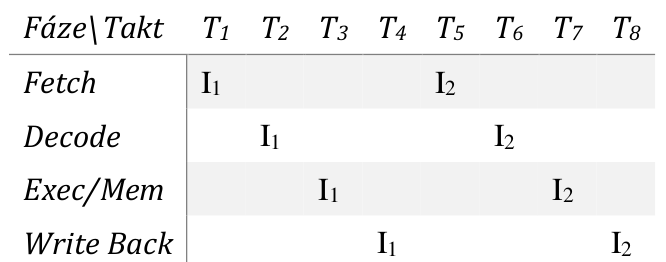
\includegraphics[width=\textwidth]{img/sekv.png}
    \end{minipage}
    \hfill
    \begin{minipage}[b]{0.4\textwidth}
        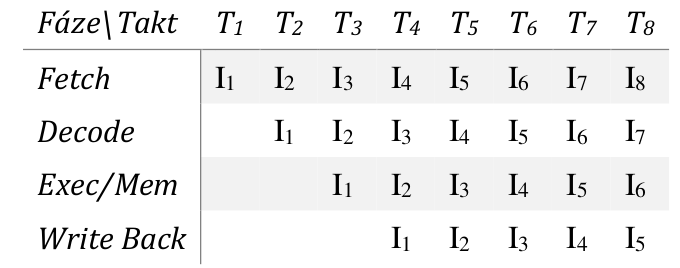
\includegraphics[width=\textwidth]{img/pipeline.png}
    \end{minipage}
\end{figure}

Doba exekuce instrukcí, kde k je počet fází:
\begin{center}
    Pipelining: $N = k + (n-1)$\\
    Sekvenční: $M = n \cdot k$ \\
    Koeficient zrychlení: $S_k = \frac{M}{N} = \frac{n \cdot k}{n + n-1}$
\end{center}

\subsection{Skokový konflikt}
Při instrukci větvení nebo přerušení. Ve chvíli kdy se začne provádět skok jsou v řetězci rozpracované instrukce. Řetězec tudíž musí být vyprázdněn a znovu naplněn, což vede ke snížení efektivity.\\
Řešení:
\begin{itemize}
    \item Predikce skoků
          \begin{itemize}
              \item Statická - nebere v úvahu historii provádění příslušné operace skoku. Například při provádění cyklu se skok provede vždy, instrukce obsahuje bit, který nastaví překladač (překladač odhaduje pravděpodobnost skoku)
              \item Dynamická - snaží se předpovědět skoky na základě chování programu v minulosti. Například provedl-li se skok při minulé exekuci dané instrukce počítá se, že se provede znovu. Procesor musí být vybaven spekulativní jednotkou
          \end{itemize}
    \item Použití dvou řetězců - 2 řetězce, jeden pro sekvenční provádění a druhý pro skoky.
\end{itemize}

\subsection{Datový konflikt}
Pokud instrukce pracuje s operandem z předchozí instrukce, která se však ještě nedokončila. \\

\begin{figure}[h!]
    \centering
    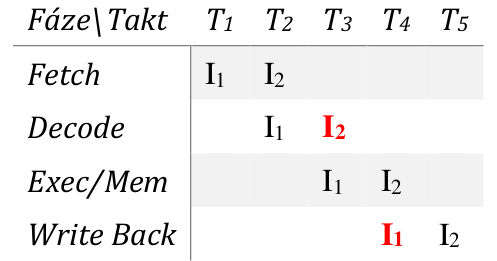
\includegraphics[scale = 0.4]{img/datKonf.png}
\end{figure}

Řešení:
\begin{itemize}
    \item Překladač řadí instrukce tak aby ke konfliktu nedošlo.
    \item Procesor detekuje konflikt a pozastaví konání $I_2$. Snižuje účinost řetězení.
    \item Procesor detekuje konflikt a změní pořadí instrukcí. Náročné na konstrukci procesoru.
\end{itemize}

\subsection{Superpipelined procesor}
Procesor rozdělený na subprocesory, které zpracovávají instrukce jako řetězec. \\
Subprocesory je možné dělit na subbloky, které tvoří řetězce subprocesorů. \\

\subsection{Mikroprocesor, mikrokontrolér, signálový procesor, signálový kontroler,SOC, ASIC}
\subsubsection{Mikroprocesor pro všeobecné využití}
Na jednom čipu ALU, řadič, registry, případně cache a MMU.\\
Velký výpočetní výkon a paměťový prostor.\\
Stolní PC, notebooky, servery.\\
Modifikace pro telefony a tablety, optimalizovány na nízkou spotřebu, nižší výkon a paměť. \\

\subsubsection*{Mikrokontrolér}
Základní stavební kámen vesvných zařízeních. \\
Na jednom čipu procesor (řadič, ALU, registry, případně cache a MMU), paměti RAM a FLASH, řadič přerušení a periferie.\\
Menší výkon a paměť.\\
Určen pro embedded aplikace, spotřební elektronika, průmysl, automobily, řídící aplikace. \\

\subsubsection*{Signálový procesor - DSP}
Vznikly pro číslicové zpracování signálů v reálném čase a spektrální analýzu. \\
Vyžadují rychlé provádění specifických výpočetních operací, ale nepotřebují moc paměti. Například multiply and accumulate, v podstatě konvoluce, součin dvou parametrů a přičtení k proměnné.\\
Méně periferií než mikrokontroléry. \\
Dělí se na 2 typy:
\begin{itemize}
    \item S pevnou řádovou čárkou - jednodušší, levnější, algoritmy se hůře implementují
    \item S plovoucí řádovou čárkou, dražší, ale jednodušší implementace
\end{itemize}

\subsubsection*{Signálový kontroler - DSC}
Kombinace DSP a mikrokontroleru.\\
Má více periferií oproti DSP. \\
Využití pro výkonovou elektroniku. Měniče, vektorové řízení motorů.\\

\subsubsection*{System on a chip - SoC}
Integrovaný obvod, který zahrnuje všechny části počítače na jeden čip. \\
Digitální, analogové, rádiové, smíšené obvody na jednom čipu. \\

\subsubsection*{ASIC}
Integrovaný obvod navržený pro jednu aplikaci.\\
Většinou digitální, hromadná výroba.\\